% 问题三
\section{问题三的模型建立与求解}

\subsection{模型准备}

\subsubsection{动作协议与时间模型}

机器狗的位置和当前频道由相邻动作的位置、频道参数唯一确定，求解过程只需维护该状态。为避免网络重试重复计入，重试沿用原 \texttt{request\_id} 与载荷，并同时校验 HTTP 状态和响应中的 \texttt{accepted} 字段；在线算法记录剩余现实时间并保留截止余量。

\subsubsection{几何证据与清除证书}

对频道 $c$ 在测站 $S$ 的一次测量结果作如下解释：

\begin{enumerate}
\item \texttt{direction}：返回正常示向度 $\hat\theta_c(S)$，用于生成示向锥；
\item \texttt{near}：测站与目标的距离不超过 $5\mathrm{m}$，可直接在测站清除；
\item \texttt{no\_signal}：当前测站不在该源的有效接收范围内，只能作为阴性证据，不能单独证明频道为空。
\end{enumerate}

频道 $c$ 的可行定位区域记为 $K_c$。在线算法以多边形外包围 $A_c$ 代替精确圆弧边界，并保持

\begin{equation}
K_c\subseteq A_c.
\label{eq:q3_outer_contain}
\end{equation}

利用问题一的半平面裁剪算法更新 $A_c$\cite{sutherland1974}。设 $C_c$ 为 $A_c$ 的覆盖圆心，定义保守半径

\begin{equation}
\rho_c=\max_{X\in A_c}\lVert X-C_c\rVert_2.
\label{eq:q3_outer_radius}
\end{equation}

由于欧氏范数是凸函数，其在凸多边形上的最大值必在顶点取得。若

\begin{equation}
\rho_c\le r_{\mathrm{opt}}-\epsilon_{\mathrm{num}},
\qquad
\epsilon_{\mathrm{num}}=0.001\mathrm{m},
\label{eq:q3_clear_certificate}
\end{equation}

则任取 $G\in K_c$，均有 $\lVert G-C_c\rVert_2\le\rho_c<20\mathrm{m}$，故在 $C_c$ 处执行的清除动作具有严格几何证书。若为衔接路径而偏移清除点，则仅当该点到 $A_c$ 全部顶点的最远距离仍不超过 $19.999\mathrm{m}$ 时执行；由 $K_c\subseteq A_c$，此时对真实源的距离证书仍然成立。若检测结果直接为 \texttt{near}，则在当前测站清除。除这两种情形外，不执行试探性清除。

\subsubsection{频道状态与终止条件}

每个频道维护一个状态，其含义如表~\ref{tab:q3_states}所示。

\begin{table}[htbp]
\centering
\small
\setlength{\tabcolsep}{3pt}
\caption{问题三频道状态及进入条件}
\label{tab:q3_states}
\begin{tabularx}{\textwidth}{@{}p{0.20\textwidth}p{0.28\textwidth}X@{}}
\toprule
状态 & 含义 & 进入条件 \\
\midrule
\texttt{unknown} & 尚未发现目标，也尚未认证为空 & 初始状态 \\
\texttt{localizing} & 已发现目标，正在收缩定位区域 & 已获得正常示向度，但尚未达到清除条件 \\
\texttt{clear\_ready} & 当前外包围已满足光学清除半径 & $\rho_c\le19.999\mathrm{m}$ \\
\texttt{cleared} & 已成功清除 & \texttt{/clear} 返回成功 \\
\texttt{absent\_certified} & 已证明频道内不存在干扰源 & 七站均实测无信号或已有严格推断，或已发现 16 源 \\
\texttt{geometry\_fault} & 定位区域为空或认证后的动作无法闭合证书 & 空区域、认证清除失败或有限覆盖仍未闭合等异常 \\
\bottomrule
\end{tabularx}
\end{table}

终止判据要求，仅当所有频道均已清除或认证为空时，才可调用一次 \texttt{/exit}。若仍存在未发现频道、定位未闭合频道或几何故障状态，则任务尚未闭合，不能报告为完成。

\subsection{模型建立}

\subsubsection{七点扫描覆盖与发现证书}

取

\begin{equation}
P_0=(0,0),
\qquad
P_k=1200\left(\cos\frac{k\pi}{3},\ \sin\frac{k\pi}{3}\right),
\quad k=1,\ldots,6.
\label{eq:q3_scan_sites}
\end{equation}

七点集合记为 $\mathcal S$。将目标圆域按六个 $60^\circ$ 扇区划分，第 $k$ 个扇区以 $P_k$ 为中心方向。对扇区内任一点 $G$，记 $r=\lVert G\rVert_2$，其相对 $P_k$ 的夹角为 $\varphi\in[-30^\circ,30^\circ]$。由于构型关于每个扇区的中线对称，只需分析 $0\le\varphi\le30^\circ$；六个扇区除旋转外完全相同。

原点与 $P_k$ 到 $G$ 的距离相等当且仅当

\begin{equation}
r=\frac{600}{\cos\varphi}.
\label{eq:q3_voronoi_boundary}
\end{equation}

若 $r\le600/\cos\varphi$，则到原点的距离不超过

\begin{equation}
\frac{600}{\cos30^\circ}=400\sqrt3\approx692.82\mathrm{m}.
\label{eq:q3_inner_bound}
\end{equation}

若 $r\ge600/\cos\varphi$，则到 $P_k$ 的平方距离关于 $r$ 是凸二次函数，其在区间 $[600/\cos\varphi,1800]$ 的端点取得最大值。径向左端点处两扫描点到 $G$ 的距离相等且不超过 $692.82\mathrm{m}$；目标圆域外端点对应的距离为

\begin{equation}
f(\varphi)
=
\sqrt{1800^2+1200^2-2\cdot1800\cdot1200\cos\varphi}.
\label{eq:q3_outer_radial}
\end{equation}

$f(\varphi)$ 在 $0\le\varphi\le30^\circ$ 上单调增加，故

\begin{equation}
d_{\max}
=f(30^\circ)
=
\sqrt{1800^2+1200^2-2\cdot1800\cdot1200\cos30^\circ}
=968.9015717\mathrm{m}.
\label{eq:q3_dmax}
\end{equation}

因此，目标圆域内任一点到 $\mathcal S$ 中最近扫描点的距离不超过 $d_{\max}$；图~\ref{fig:q3_scan_certificate}给出了扫描点、接收圆盘与最坏边界位置的关系。

\begin{figure}[htbp]
\centering
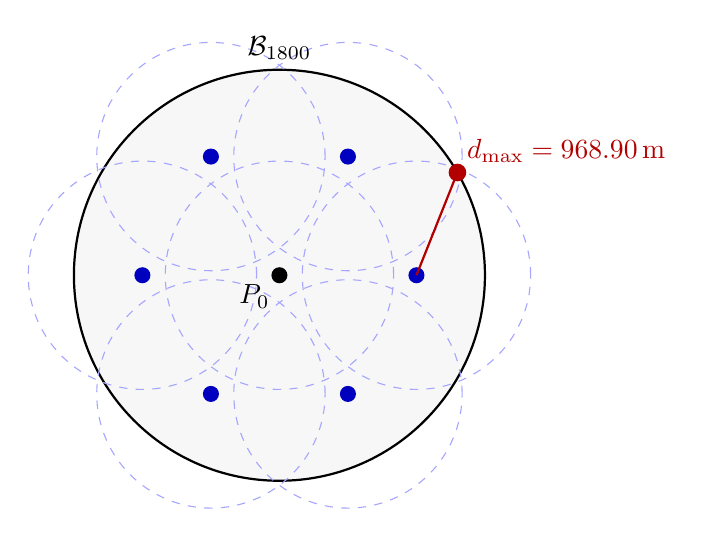
\begin{tikzpicture}[scale=1.45]
  \fill[black!3] (0,0) circle (1.8);
  \draw[thick] (0,0) circle (1.8);
  \draw[blue!35,dashed] (0,0) circle (1.0);
  \fill[black] (0,0) circle (2pt);
  \foreach \k in {0,...,5}{
    \coordinate (Q\k) at ({1.2*cos(60*\k)},{1.2*sin(60*\k)});
    \draw[blue!35,dashed] (Q\k) circle (1.0);
    \fill[blue!75!black] (Q\k) circle (2pt);
  }
  \coordinate (W) at ({1.8*cos(30)},{1.8*sin(30)});
  \fill[red!70!black] (W) circle (2.2pt);
  \draw[red!70!black,thick] (Q0)--(W);
  \node[above] at (0,1.8) {$\mathcal B_{1800}$};
  \node[below left] at (0,0) {$P_0$};
  \node[above right,red!70!black] at (W) {$d_{\max}=968.90\,\mathrm m$};
\end{tikzpicture}
\caption{问题三七点扫描骨架、接收覆盖与最坏位置}
\label{fig:q3_scan_certificate}
\end{figure}

\textbf{命题 1（发现完备性）}　若 $1000\mathrm{m}\le r_j^{\mathrm{recv}}\le1500\mathrm{m}$，则每个干扰源在七个扫描点中至少一个点上会被检测到；若某频道在七个扫描点上均返回 \texttt{no\_signal}，则该频道必不存在干扰源。

证明：由 $d_{\max}<1000\mathrm{m}$，任一干扰源到最近扫描点的距离不超过 $968.9016\mathrm{m}$，位于其有效接收范围内。由于问题三中的干扰源为全向源，该点不会出现方向盲区，因此测量结果只能是 \texttt{direction} 或 \texttt{near}。反之，若七个点均无信号，则与上述必然有信号矛盾。证毕。

七个扫描点构成发现证书，其正确性只依赖扫描点的集合，与访问顺序无关。因此，后续为缩短路径而重排扫描站不会削弱该证书。

若某频道已经获得一次有效响应，则记为“已发现源”；同一频道的多次观测只对应一个源。当已发现不同频道数达到 16 时，根据干扰源总数不超过 16 以及频道唯一性，剩余频道必为空，可直接认证为 \texttt{absent\_certified}。该结论可缩短扫描过程，且不需要额外的阴性观测。

\subsubsection{阴性证据推理}

设 $Q$ 是频道 $c$ 的一个无信号站，$S$ 是尚未测量但可接收该源的候选站，并记该源的有效接收半径为 $r^{\mathrm{recv}}$。若目标 $G$ 在 $S$ 处可接收而在 $Q$ 处不可接收，则

\begin{equation}
\lVert G-S\rVert_2\le r^{\mathrm{recv}}<\lVert G-Q\rVert_2.
\label{eq:q3_negative_order}
\end{equation}

平方后可得

\begin{equation}
(Q-S)^{\mathsf T}G
<
\frac{\lVert Q\rVert_2^2-\lVert S\rVert_2^2}{2}.
\label{eq:q3_negative_halfplane}
\end{equation}

右端等于 $(Q-S)^{\mathsf T}(Q+S)/2$，因此上式定义一个开半平面。将其与目标圆域、距离上界以及其余无信号站产生的不等式求交，若交集为空，则候选站 $S$ 不可能接收该源，扫描时可直接跳过并记为推断无信号。

另一种阴性证据来自圆盘覆盖：设候选区域被若干已测得无信号站周围半径 $1000\mathrm{m}$ 的圆盘覆盖。若源位于该区域，则它到某个无信号站的距离不超过 $1000\mathrm{m}\le r^{\mathrm{recv}}$，该站本应收到信号，与事实矛盾。因此，只要连续区域的圆盘覆盖关系成立，即可安全跳过相应测量。推断阴性只用于更新认证状态，不记录为实际测量结果。

\subsubsection{保证有信号的第二测站}

设首次正常示向度为 $\hat\theta$，其单位方向为 $d=d(\hat\theta)$，左法向量为 $d^{\perp}=d^{\perp}(\hat\theta)$。取

\begin{equation}
S'=S+400d+300d^{\perp}.
\label{eq:q3_safe_site}
\end{equation}

该点与首点的距离为 $500\mathrm{m}$，相对首条视线的横向偏移为 $300\mathrm{m}$。

设首点测得方向时源距为 $r$，真实方向与名义方向的夹角为 $\varepsilon_\theta$，满足 $|\varepsilon_\theta|\le\delta_{\mathrm{num}}$。位移向量 $w=S'-S=400d+300d^{\perp}$，令 $a=w\cdot d(\hat\theta+\varepsilon_\theta)$，则

\begin{equation}
a
=400\cos\varepsilon_\theta+300\sin\varepsilon_\theta
\ge400\cos\delta_{\mathrm{num}}-300\sin\delta_{\mathrm{num}}
>394.6\mathrm{m}.
\label{eq:q3_projection_bound}
\end{equation}

因此

\begin{equation}
\begin{aligned}
\lVert G-S'\rVert_2^2
&=r^2+500^2-2ra\triangleq\Phi(r).
\end{aligned}
\label{eq:q3_distance_change}
\end{equation}

$\Phi(r)$ 是开口向上的二次函数。若 $r\ge1000\mathrm{m}$，则由 $a>394.6\mathrm{m}$ 得 $250000-2ar<0$，故 $\lVert G-S'\rVert_2<r\le r^{\mathrm{recv}}$。若 $r<1000\mathrm{m}$，则 $\Phi$ 在 $[0,1000]$ 上的最大值必在端点取得，而
\[
\Phi(0)=500^2<1000^2,
\qquad
\Phi(1000)=1000^2+500^2-2000a<1000^2.
\]
因此 $\lVert G-S'\rVert_2<1000\mathrm{m}\le r^{\mathrm{recv}}$。综上，$S'$ 必能收到该源的有效响应。该构造只改变测量位置，不增加误差分布假设。

\subsubsection{定位区域更新与测站选择}

初始化频道 $c$ 的外包围为覆盖目标圆域的正多边形。获得正常示向度后，依次执行：

\begin{enumerate}
\item 用 $\delta_{\mathrm{num}}$ 生成示向锥 $W(S,\hat\theta_c)$ 的两条半平面；
\item 与外包围 $A_c$ 求交；
\item 用 $\lVert G-S\rVert_2\le1500\mathrm{m}$ 的圆域支撑半平面继续裁剪；
\item 对每个无信号站 $Q\in\mathcal D_c$，用半平面 $R(Q,S)$ 排除不可能位置；
\item 重新计算外包围的覆盖圆心 $C_c$ 和保守半径 $\rho_c$。
\end{enumerate}

若 $A_c$ 为空，则报告观测矛盾；若 $\rho_c\le19.999\mathrm{m}$，则转入清除；否则继续选择新测站。正常测站候选满足以下条件：

\begin{enumerate}
\item 具有接收保证：候选点到当前外包围中任一点的距离均小于 $999.99\mathrm{m}$，对应数学上的严格接收保证，并保留 $0.01\mathrm{m}$ 的数值余量；或候选点到该外包围中每一点的距离都严格小于某个既有成功观测站到相应点的距离，从而利用首次成功接收所给出的接收半径下界；
\item 候选点到当前外包围的最远距离不超过 $1499.99\mathrm{m}$，从而除非目标距候选点不超过 $5\mathrm{m}$ 并转入 \texttt{near} 清除，否则返回的方向必为有效 \texttt{direction}；
\item 名义方位预评估显示其能使定位半径下降；
\item 当 $\rho_c\le450\mathrm{m}$ 时，对可能返回的方位按不超过 $2^\circ$ 分箱，并对每个分箱扩大误差半角后计算裁剪区域半径上界；优先选择上界不超过 $19.5\mathrm{m}$ 或小于当前半径 $75\%$ 的测站。若不存在这样的改进候选，则回到基础候选规则，不把启发式上界误当成可行性硬约束。
\end{enumerate}

最后一项使用误差上界而非名义方位做决策，避免因未知返回值导致测站选择乐观失效。所有候选步骤仍以问题一的半平面交和最小覆盖圆为几何内核。

当 $\rho_c\le300\mathrm{m}$ 时，采用十二点环形测站包：

\begin{equation}
a_c=1.2\rho_c+8,
\qquad
S_i=C_c+a_c\left(\cos\psi_i,\sin\psi_i\right),
\quad
\psi_i=\psi_0+\frac{i\pi}{6}.
\label{eq:q3_packet_sites}
\end{equation}

任一测站到可能源的距离不超过

\begin{equation}
a_c+\rho_c=2.2\rho_c+8\le668\mathrm{m},
\label{eq:q3_packet_receive}
\end{equation}

故十二个测站均有信号保证。十二个方位均匀分布的测站用于改善交会几何，是否继续访问仍由保守半径的实际收缩判定。每轮最多访问十二个环点；一旦半径降至本轮初始值的 $55\%$ 以下或达到清除阈值，本轮提前结束。外层在 $\rho_c\le300\mathrm{m}$ 时最多重复 8 轮，每轮均按更新后的 $C_c$ 和 $\rho_c$ 重建测站包；若仍不足以达到清除阈值，则转入有限覆盖兜底。

\subsubsection{有限覆盖清除与完备性}

当快速定位分支停滞时，对当前外包围 $A_c$ 进行递归细分。每次沿投影跨度较大的方向将单元二分，直到每个叶单元的保守半径不超过

\begin{equation}
\varepsilon_{\mathrm{cov}}=4.5\mathrm{m}.
\label{eq:q3_cover_radius}
\end{equation}

对单元中心 $S$ 执行一次检测。若真实源位于该单元，则

\begin{equation}
\lVert G-S\rVert_2\le\varepsilon_{\mathrm{cov}}<5\mathrm{m},
\label{eq:q3_near_guarantee}
\end{equation}

测量结果必为 \texttt{near}，随后在该点执行光学清除。保证测站若返回 \texttt{no\_signal}，说明该观测与接收保证证书冲突；算法不会将任务直接判为成功，而是结束当前快速分支并进入本有限覆盖过程。只有有限覆盖完成后仍未取得合法清除证书时，才报告几何故障。

覆盖细分只保留与当前外包围仍有交集的单元，而真实源始终属于当前外包围，因此真实源所在叶单元不会被丢弃。单元半径按全部顶点到覆盖圆心的最大距离保守计算；每次对当前较大投影跨度作二分，随着单元尺寸收缩，有限步内即可达到 $4.5\mathrm{m}$。该分支不依赖空清除；若数值退化导致单元覆盖无法推进，算法报告几何故障，而不是假定清除成功。

综上，在本章假设下，每个实际存在的全向干扰源都能被发现并最终获得合法清除路径；每个未发现频道也都有实测 \texttt{no\_signal}、严格阴性推断或 16 源上界之一作为认证依据。因此，终止时不会出现未闭合频道。

\subsubsection{联合路径调度模型}

在时间表达式中，单次检测、换频和清除的时间固定，主要可控项为总移动距离 $L$。设当前重规划时刻的必选任务节点集为

\begin{equation}
V_t=V_t^{\mathrm{scan}}\cup V_t^{\mathrm{service}},
\label{eq:q3_task_nodes}
\end{equation}

其中 $V_t^{\mathrm{scan}}$ 为尚未完成必要阴性认证的扫描站，$V_t^{\mathrm{service}}$ 为已完成发现但仍需定位或清除的频道服务点。后者以该频道当前的保守覆盖圆心 $C_c$ 作为规划位置。对由 $n_t$ 个节点组成的访问顺序 $\sigma=(\sigma_1,\ldots,\sigma_{n_t})$，开放路径长度定义为

\begin{equation}
L(\sigma)
=
\lVert P_{\sigma_1}-P_{\mathrm{cur}}\rVert_2
+
\sum_{i=1}^{n_t-1}
\lVert P_{\sigma_{i+1}}-P_{\sigma_i}\rVert_2,
\label{eq:q3_open_path}
\end{equation}

其中 $P_{\mathrm{cur}}$ 为当前机器狗位置，开放路径不要求返回起点。当前节点集上的调度子问题为

\begin{equation}
\min_{\sigma}\quad L(\sigma).
\label{eq:q3_route_problem}
\end{equation}

节点数不超过 10 时，采用 Held--Karp 动态规划求精确开放路径。令 $d_{ij}$ 为节点间距离，状态 $F_{\mathrm{path}}(M,j)$ 表示从当前点出发访问集合 $M$ 且最后位于 $j$ 的最短距离，则

\begin{equation}
F_{\mathrm{path}}(M,j)
=
\min_{i\in M\setminus\{j\}}
\left[
F_{\mathrm{path}}(M\setminus\{j\},i)+d_{ij}
\right],
\qquad
F_{\mathrm{path}}(\{j\},j)=d_{\mathrm{cur},j}.
\label{eq:q3_held_karp}
\end{equation}

节点数超过 10 时，计算量显著上升，故先以最小增量插入构造初始解，并加入 3 个最近邻起点，再交替执行 2-opt 逆向交换和 Or-opt 邻域重定位直至无改善。此时只声称得到高质量可行路径，不声称是全局最优解。

在每个扫描站内部，除必需的未知频道外，还可在联合调度预测成本较低的条件下，顺势补测已发现且尚未达到清除精度的频道。仅当预期定位半径明显下降，且预计节省的往返时间超过本次测量与换频成本时，才将该测量加入站内任务；否则留给后续必经站处理。该“顺路收获”不改变动作次数的下限，但可减少为同一频道多次往返。

每完成一个联合路径节点（一次扫描站访问或一个频道的服务过程）后，在线算法重新更新频道状态、删除已闭合的扫描站或服务点，并再次求解当前节点集上的开放路径。动态重规划使后续路径能够利用新增方位和清除结果，但不改变七点发现证书。

\subsubsection{算法流程}

上述证书与动态调度合并为下面的在线闭环。伪代码只调用前文已经定义的几何算子；其中
$\operatorname{Update}_3$ 按响应分别执行示向锥裁剪、阴性证据更新或近距清除，
$\operatorname{Certify}_3$ 仅依据完整七点证书或已发现 16 个异频源关闭未知频道。

\begin{mdframed}[
  nobreak=true,
  linewidth=0.6pt,
  innerleftmargin=7pt,
  innerrightmargin=7pt,
  innertopmargin=5pt,
  innerbottommargin=2pt,
  skipabove=6pt,
  skipbelow=6pt
]
\textbf{算法 1\quad 问题三证书驱动联合调度}
\begin{tabbing}
00\quad\=\quad\quad\=\quad\quad\=\kill
1 \> 构造七点扫描集，调用一次 \texttt{/enter}；初始化频道轨迹 $T_c$、$U\leftarrow\mathcal S$、$P\leftarrow O$；\\
2 \> \textbf{while} 存在未闭合频道 \textbf{do}\\
3 \>\> $\operatorname{Certify}_3(T,U)$，并用阴性圆盘覆盖推断可安全退役的扫描站；\\
4 \>\> $V\leftarrow V^{\rm scan}(U)\cup V^{\rm service}(T)$，$a\leftarrow\operatorname{First}(\operatorname{JointRoute}(P,V))$；\\
5 \>\> \textbf{if} $a$ 不存在 \textbf{then break}；\\
6 \>\> \textbf{if} $a$ 为扫描站 $S_i$ \textbf{then}\\
7 \>\>\> $U\leftarrow U\setminus\{S_i\}$，按“必测频道 $\cup$ 有严格净收益频道”的顺序检测；\\
8 \>\>\> 对每个响应 $y$ 执行 $\operatorname{Update}_3(T_c,S_i,y)$，随后重新认证频道；\\
9 \>\> \textbf{else}\quad 令 $c$ 为服务频道，在保证接收的候选点中最小化移动与误差代价；\\
10\>\>\> 最多自适应检测 10 次；若连续两次收缩不足或返回无信号，则停止该层；\\
11\>\>\> 若 $\rho_c\le300\,\mathrm m$ 仍未闭合，则至多执行 8 轮 12 点测站包；\\
12\>\>\> 若 $\rho_c\le19.999\,\mathrm m$，在通过顶点距离证书的位置调用 \texttt{/clear}；\\
13\>\>\> 否则将 $A_c$ 细分为半径不超过 $4.5\,\mathrm m$ 的单元，逐中心检测至近距或半径证书清除；\\
14\>\> \textbf{end if}；若兜底耗尽仍未闭合，则置为 \texttt{geometry\_fault} 并停止；\\
15\> \textbf{end while}；核验 20 个频道均为 \texttt{cleared} 或 \texttt{absent\_certified}；\\
16\> 核验清除数属于 $[10,16]$，仅调用一次 \texttt{/exit}。
\end{tabbing}
\end{mdframed}

\subsection{模型求解与结果分析}

\subsubsection{计算参数}

在线计算采用 $\delta_{\mathrm{num}}=1.01^\circ$ 作为安全半角。目标圆域初始外包围采用 360 条支撑半平面，距离圆域采用 128 条支撑半平面，清除半径使用 $19.999\mathrm{m}$ 的保守阈值。七点发现骨架的最大覆盖距离为 $968.9016\mathrm{m}$，距有效接收半径下界仍有

\begin{equation}
1000-968.9016=31.0984\mathrm{m}
\label{eq:q3_cover_margin}
\end{equation}

的余量。该余量保证了在最不利接收半径下，扫描骨架仍能产生阴性认证。所有几何判断均使用外包围和保守半径，因而数值误差不会使真实源被排除在可行区域之外。

\subsubsection{演练效果}

未提速基础版共完成 18 局演练，平均定位清除时间为 $507.91\mathrm{s}$/源，所有实际干扰源均被清除且清除失败为 0。
完全提速策略定型后共完成 18 局演练，合计清除 $240/240$ 个实际干扰源，清除失败 0 次；逐局平均每源时间的等权均值为 $263.29\mathrm{s}$/源，中位数为 $258.34\mathrm{s}$/源，范围为 $197.43$--$325.96\mathrm{s}$/源，相对基础版平均值降低 $48.16\%$。
该 18 局跨越算法定型后的两个冻结构建，差异仅用于提交封装和代码整理，均采用本文的联合选路、站内顺路收获与测站选择策略，故按“完全提速版”统一统计，不再单列中间版本。基础版与完全提速版共用相同的发现、定位和清除证书，因此该对照反映的是路径与观测调度带来的效率收益。

\subsubsection{正式测试结果}

三次正式测试与其同期演练使用同一构建，提交版本在去冗余注释、文件名版本对齐与输出消息英文字符化后哈希为 \texttt{d936031c54075554}（在线决策模块 SHA-256 前 16 位）。结果如表~\ref{tab:q3_formal}所示。

\begin{table}[htbp]
\centering
\caption{问题三正式测试结果}
\label{tab:q3_formal}
\begin{tabular}{lrrr}
\toprule
测试案例编码 & 清除干扰源个数 & 平均定位清除时间/s & 程序运行时间/ms \\
\midrule
T5JT-TE93-CQUC-FDAD & 12 & 384.94 & 2401 \\
FX3P-PUBX-QE4N-783K & 13 & 220.50 & 2198 \\
Y4HS-EJMD-CXRP-BV5W & 15 & 264.31 & 2404 \\
\midrule
合计（三次按局平均） & 40 & 289.91 & 2198--2404 \\
\bottomrule
\end{tabular}
\end{table}

表中汇总行的 40 为三次清除数之和；$289.91\mathrm{s}$ 为三次单局平均定位清除时间的等权算术平均，按日志未舍入值计算得到。若改用总体合并口径，则三次总虚拟时间与总清除数之比为 $11450.33/40=286.26\mathrm{s}$/源。两种口径含义不同，本章按三次单局等权汇总，采用前者。
三次正式测试共清除 40 个干扰源，三次均无空清除。每局的 20 个频道最终均为已清除或认证为空状态，没有未知频道残留。由命题 1 的发现完备性，所有被判为不存在的频道必无干扰源；因此三次测试的清除个数均等于实际源数，被清除干扰源个数比例为 $100\%$。

三次正式测试合计移动距离为 $46.49\mathrm{km}$，虚拟总时间之和为 $11450.33\mathrm{s}$。时间构成如表~\ref{tab:q3_time}所示。

\begin{table}[htbp]
\centering
\caption{问题三三次正式测试的合计时间构成}
\label{tab:q3_time}
\begin{tabular}{lrr}
\toprule
时间项 & 数值/s & 占比 \\
\midrule
移动时间 & 9297.33 & $81.20\%$ \\
检测时间 & 1640.00 & $14.32\%$ \\
换频时间 & 313.00 & $2.73\%$ \\
成功清除时间 & 200.00 & $1.75\%$ \\
失败清除时间 & 0.00 & $0.00\%$ \\
\midrule
合计 & 11450.33 & $100.00\%$ \\
\bottomrule
\end{tabular}
\end{table}

移动时间占比超过八成，说明路径长度仍是总时间的主导因素。正式测试第 1 局的平均时间较高，主要原因是该局干扰源分布较分散，移动里程为 $19.41\mathrm{km}$，移动时间占总时间的 $84.0\%$；另两局的移动时间占比分别为 $76.3\%$ 和 $81.4\%$。这与演练批次的统计一致，表明差异主要来自案例空间分布。

程序运行时间保持在 $2198$ 至 $2404\mathrm{ms}$，远小于 $1200\mathrm{s}$ 的现实运行时上限。依据三局正式日志中的动作序列逐项复核：清除数与清除成功次数一致，检测次数和换频次数均可由动作序列复算；按四项时间分量独立重算的总时间与日志记录的虚拟时间残差不超过 $3.1\times10^{-6}\mathrm{s}$。因此，正式测试的数值结果与动作序列及时间统计一致。

从模型层面看，问题三的求解没有依赖干扰源真值或有效接收半径的先验观测。发现阶段依靠七点覆盖证书，定位阶段依靠外包围与严格清除判据，调度阶段只利用已经发生的位置、频道和测量结果。在题目给定场景及已完成测试样本中，结果支持“覆盖认证优先、批量定位清除、动态联合选路”策略的可行性与可复现性；但这组实验本身不构成对全部随机案例最优性的证明。
